\begin{frame}{Animaciones del sistema}
  \begin{columns}[T]
    \begin{column}{0.48\textwidth}
      \centering{\small $N = 100$}\par
      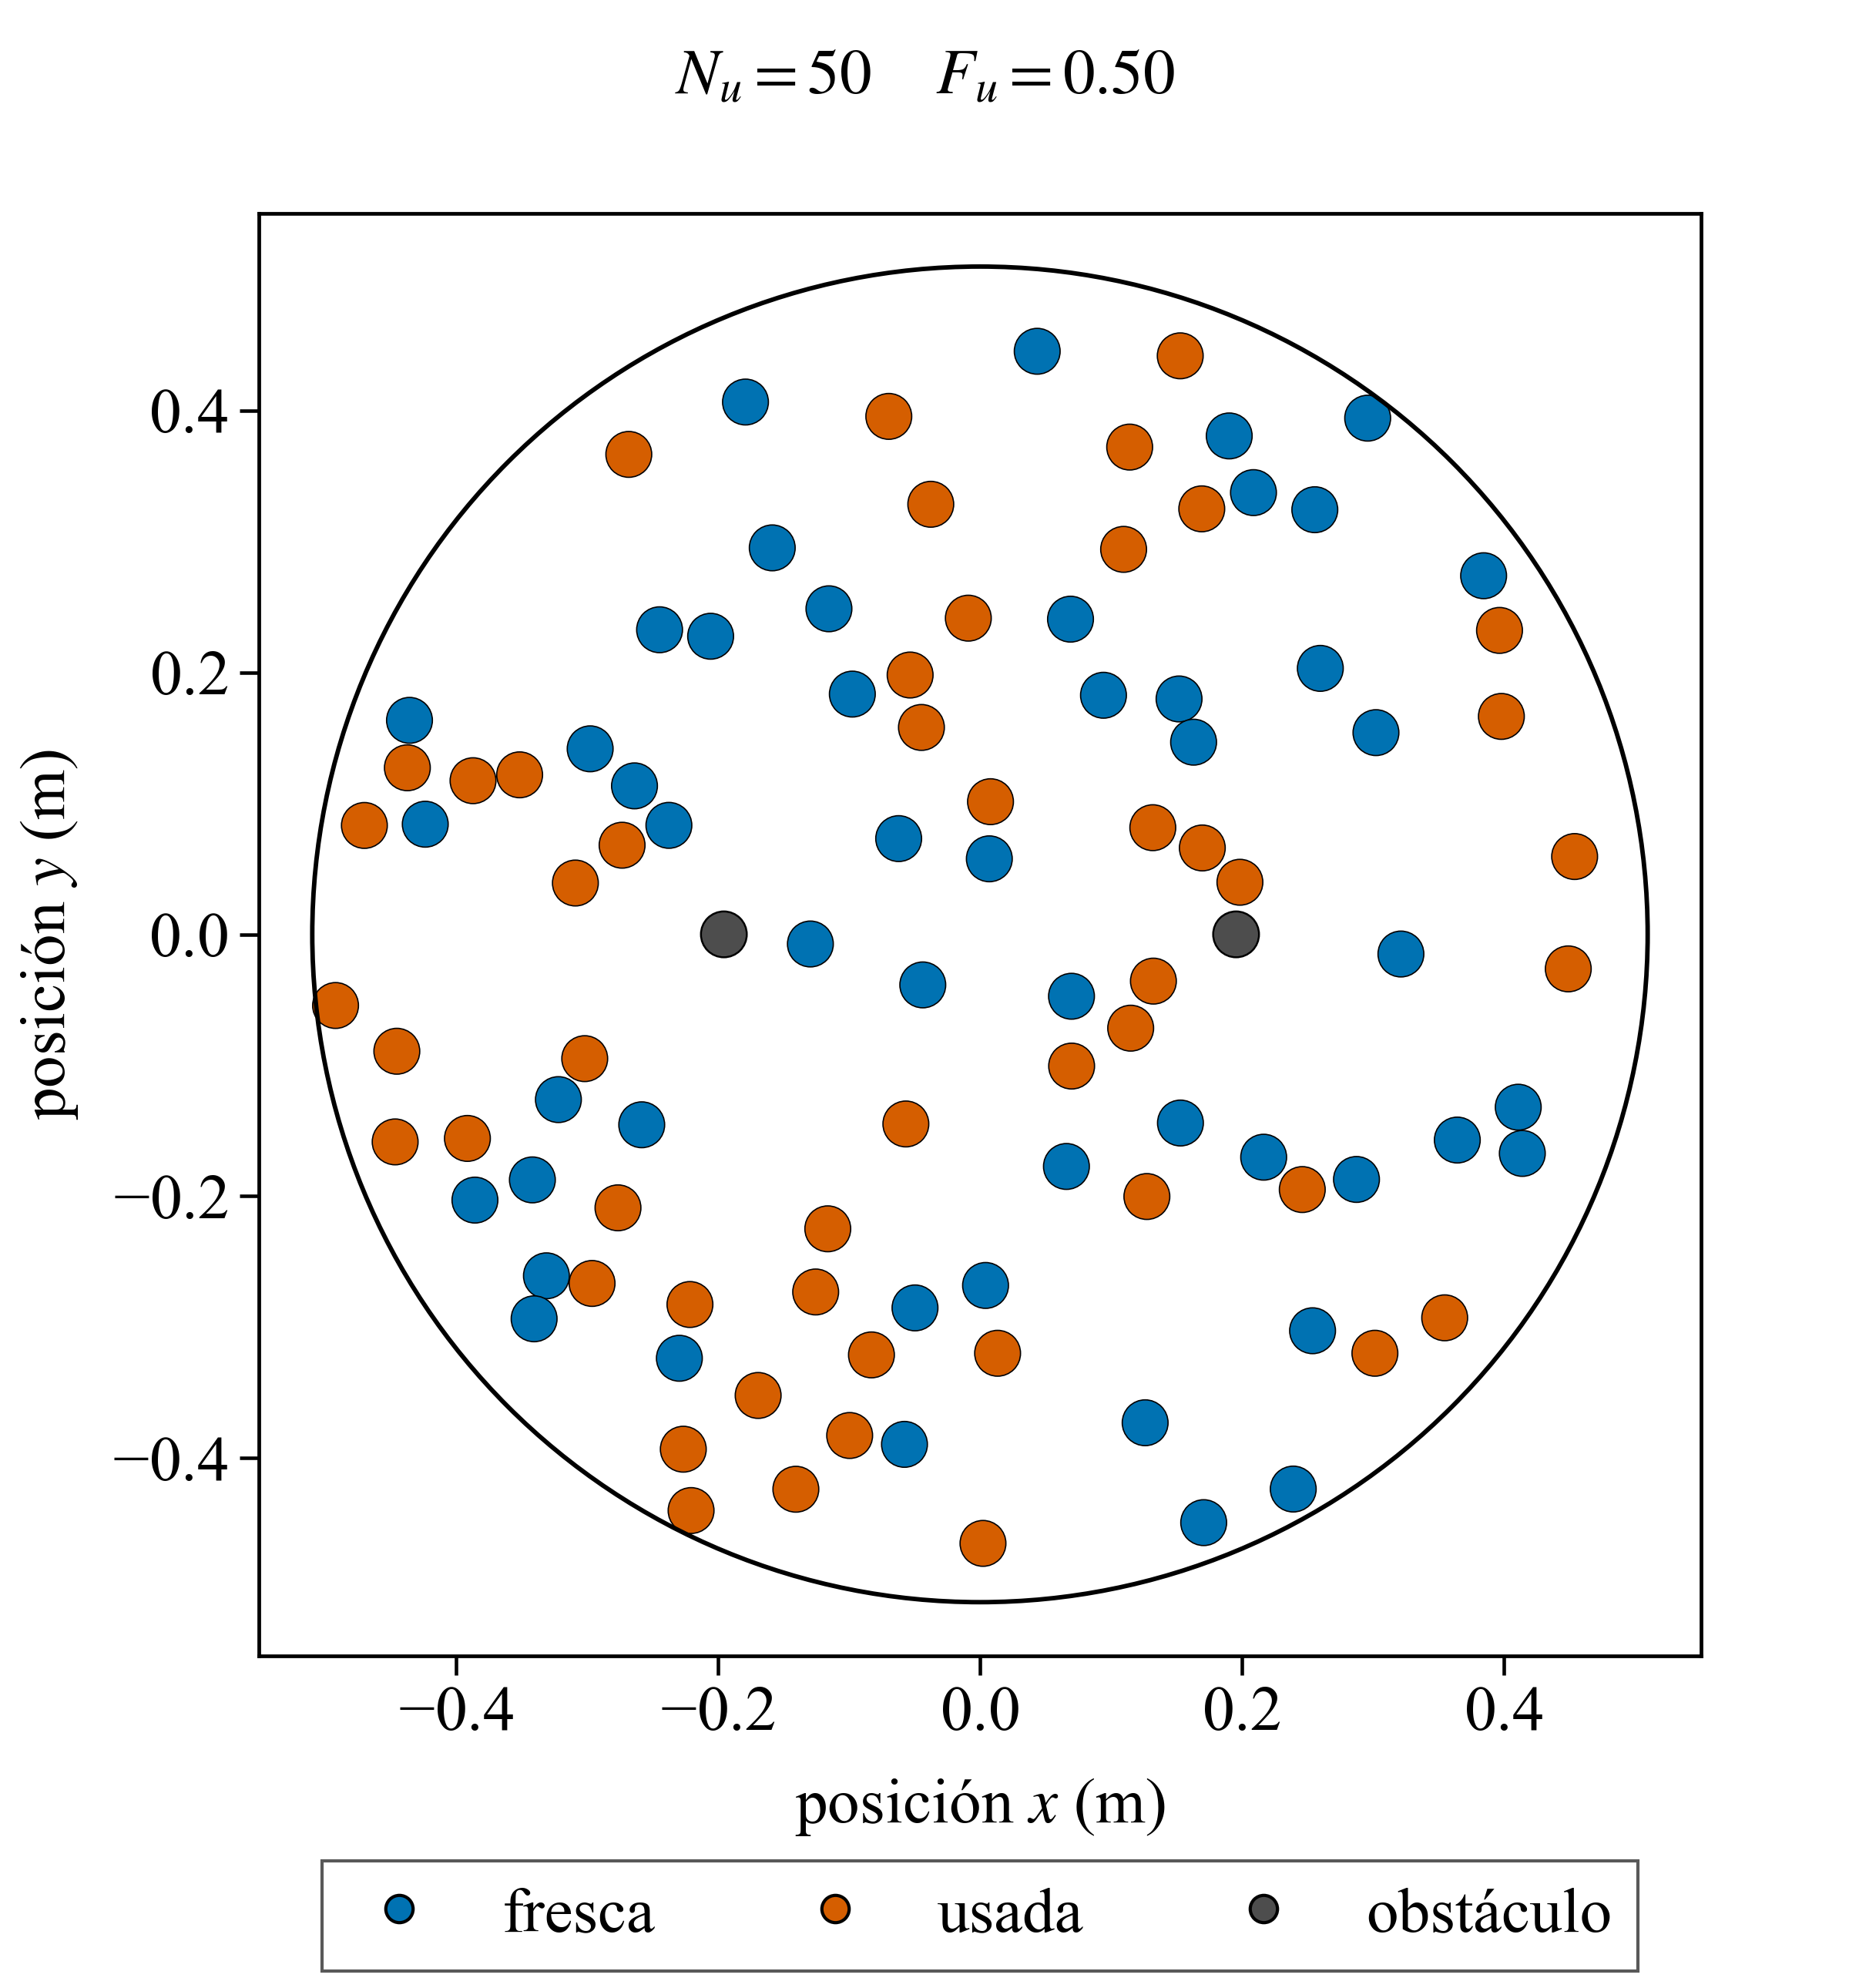
\includegraphics[width=\linewidth,height=0.78\textheight,keepaspectratio]{anim_N100.png}
    \end{column}
    \begin{column}{0.48\textwidth}
      \centering{\small $N = 20$}\par
      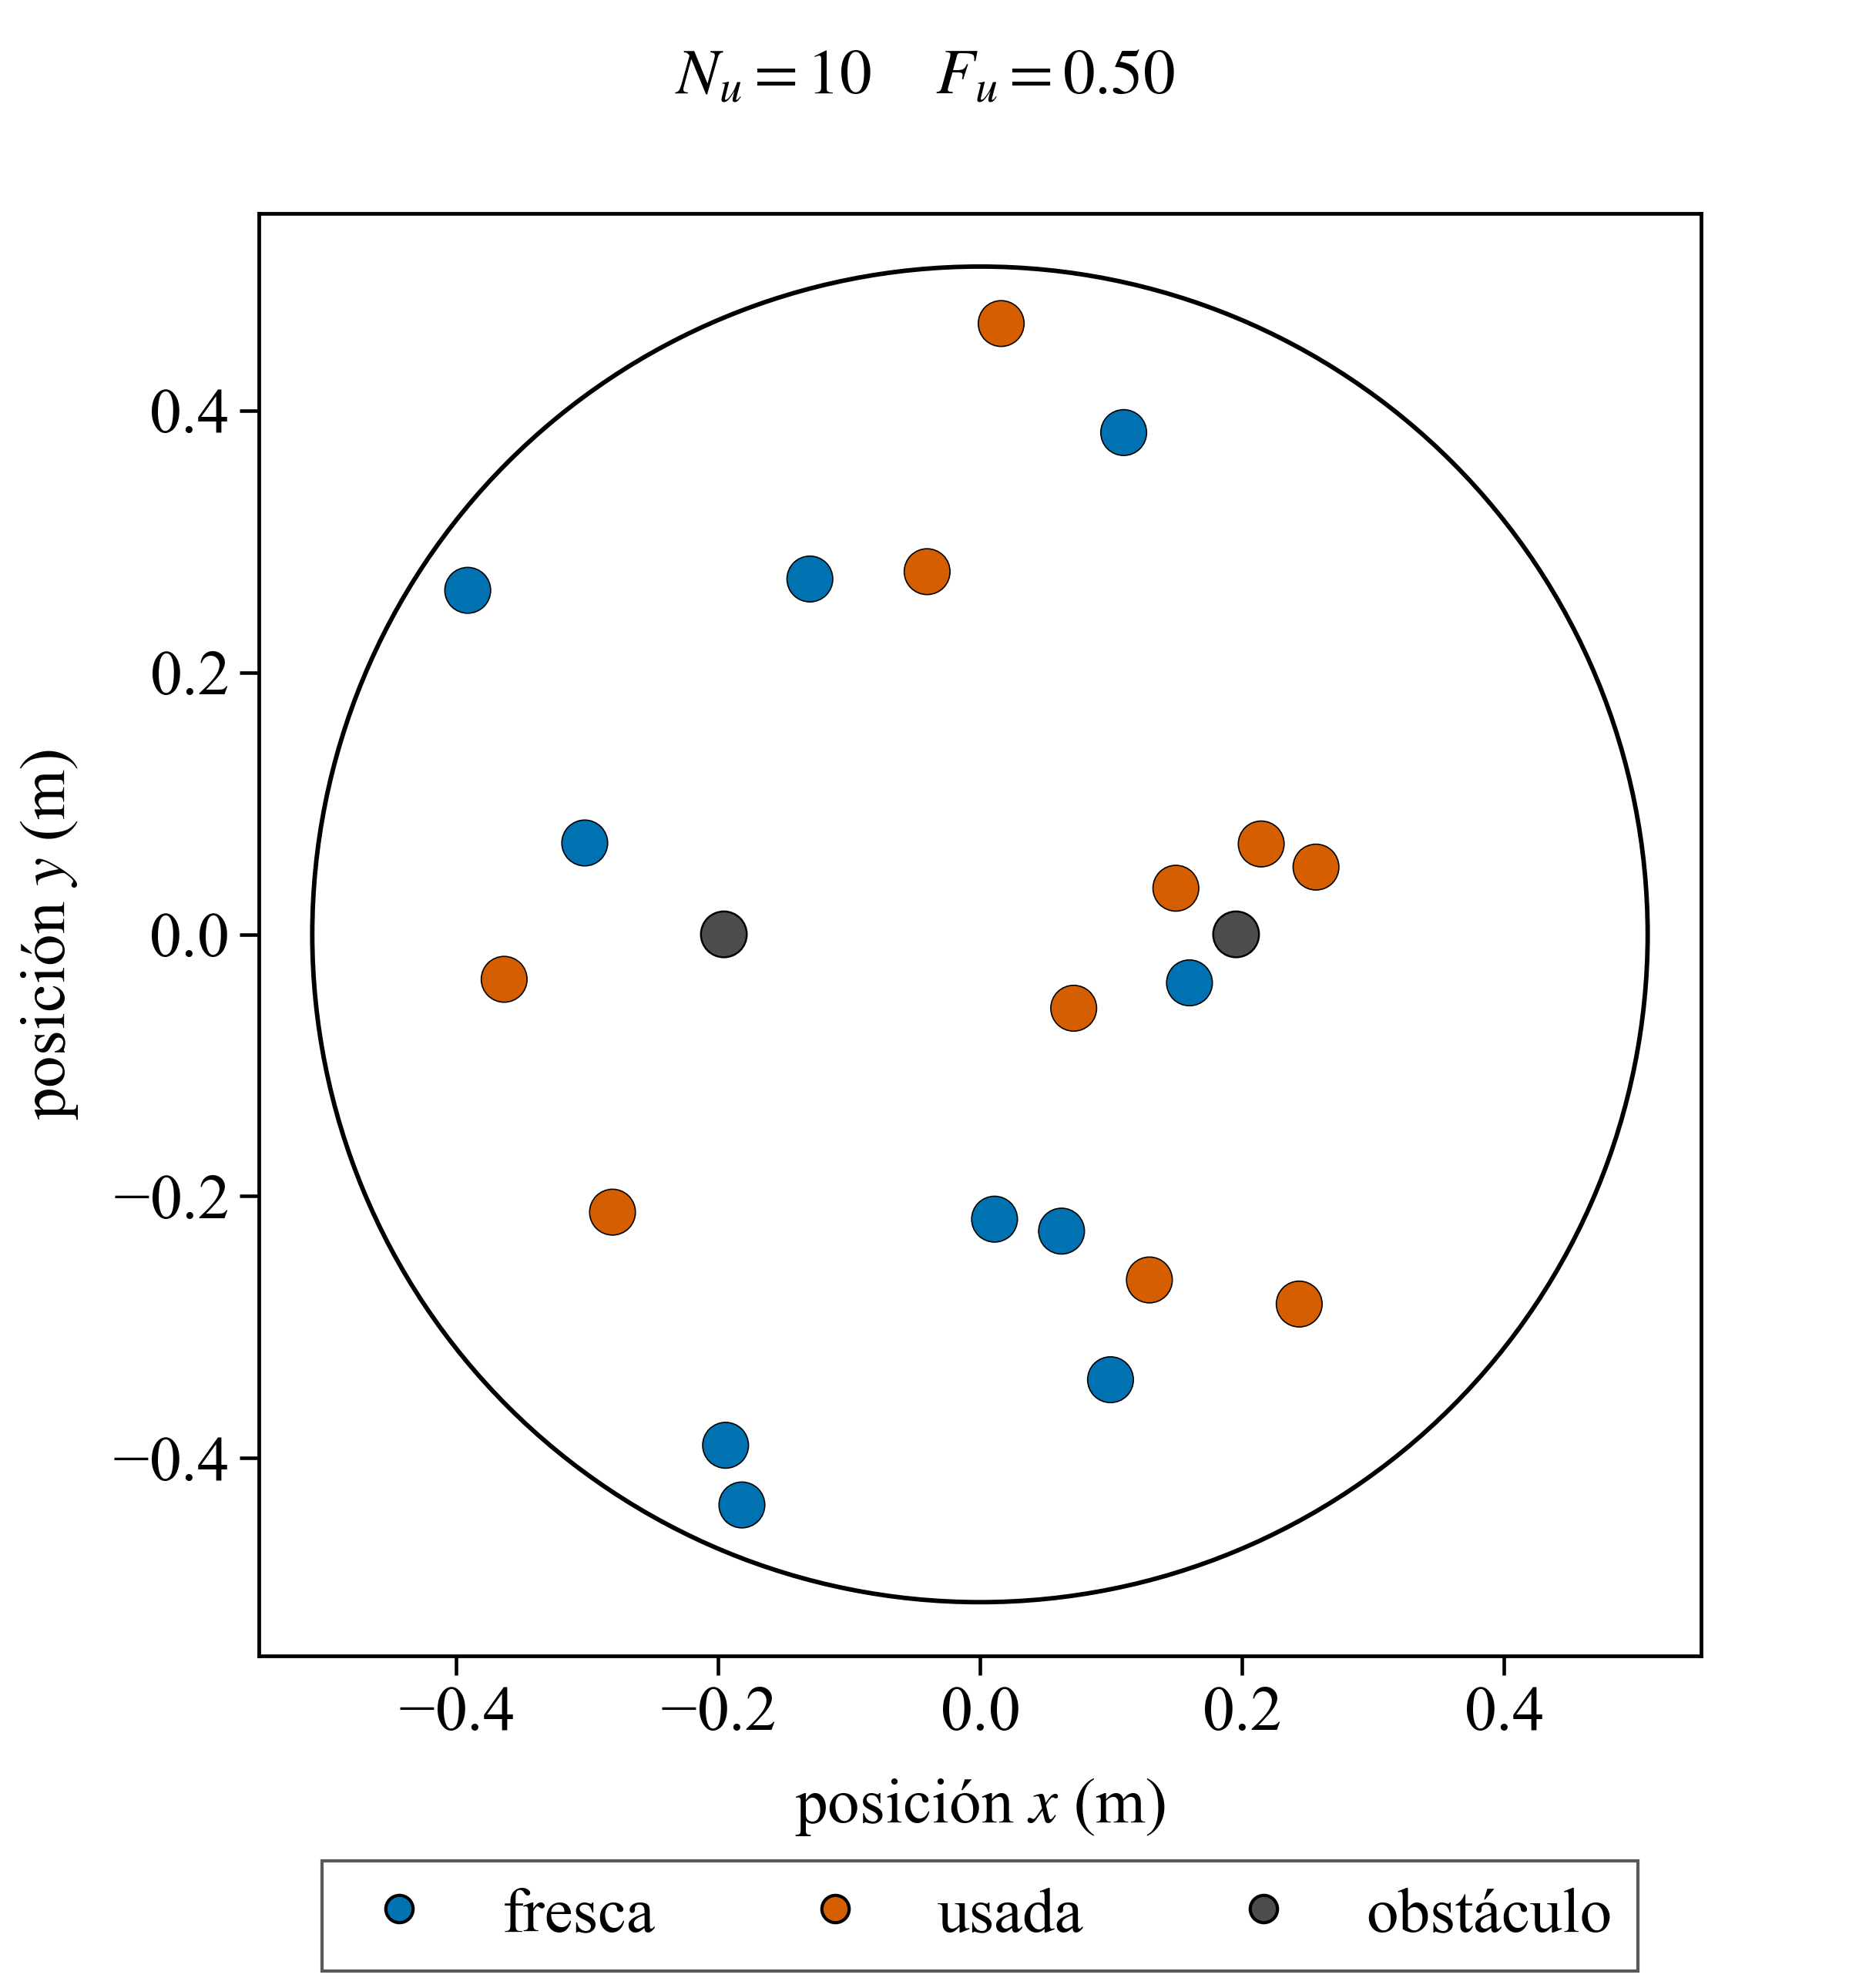
\includegraphics[width=\linewidth,height=0.78\textheight,keepaspectratio]{anim_N20.png}
    \end{column}
  \end{columns}
\end{frame}

\begin{frame}{Fracción de partículas usadas}
  \begin{cols}
    \begin{column}{0.62\textwidth}
      \figura{fu_N100.png}
    \end{column}
    \begin{column}{0.34\textwidth}
      \begin{parametros}
        \item $N = 100$
      \end{parametros}
      \begin{resultado}
        \item $x_o = 0.196\uni{m}$
        \item $\langle t_{90}\rangle = 14.99 \pm 1.71\uni{s}$
      \end{resultado}
    \end{column}
  \end{cols}
\end{frame}

\begin{frame}{$\langle t_{90}\rangle$ en función de $x_o$}
  \begin{cols}
    \begin{column}{0.62\textwidth}
      \figura{t90_vs_xo.png}
    \end{column}
    \begin{column}{0.34\textwidth}
      \begin{parametros}
        \item $t_{\max} = 100\uni{s}$
        \item $30$ realizaciones
        \item $x_o$ de $r$ a $R - r$
      \end{parametros}
      \begin{resultado}
        \item $N = 100$: $x_o = 0.196\uni{m}$, $14.99 \pm 1.71\uni{s}$
        \item $N = 20$: $x_o = 0.255\uni{m}$, $11.69 \pm 2.80\uni{s}$
      \end{resultado}
    \end{column}
  \end{cols}
\end{frame}
